\documentclass[a4paper,12pt,twocolumn]{article}
\usepackage{graphicx}
\usepackage[margin=0.5in]{geometry}
\usepackage[cmex10]{amsmath}
\usepackage{array}
\usepackage{gensymb}
\usepackage{booktabs}
\usepackage{tabularx}
\title{Line Assignment}

\author{Ginna Shreyani- FWC22006}
\date{September 2022}
\providecommand{\norm}[1]{\left\lVert#1\right\rVert}
\providecommand{\abs}[1]{\left\vert#1\right\vert}
\let\vec\mathbf
\newcommand{\myvec}[1]{\ensuremath{\begin{pmatrix}#1\end{pmatrix}}}	
\newcommand{\mydet}[1]{\ensuremath{\begin{vmatrix}#1\end{vmatrix}}}
\providecommand{\brak}[1]{\ensuremath{\left((#1\right)}}
\begin{document}
\maketitle
\section{Problem:}
Diagonal AC of a parallelogram ABCD bisects $\angle{A}$. Show that \\
(i) it bisects $\angle{C}$\\
\begin{figure}[h]
	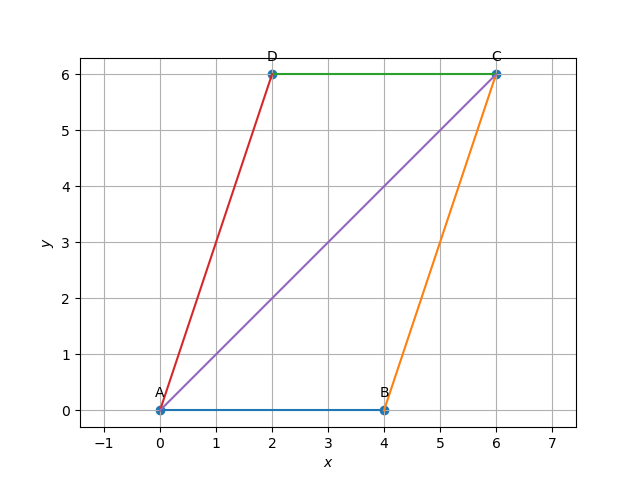
\includegraphics[width=\linewidth]{parallel.png}
\end{figure}
\maketitle
\section{Construction:}
\begin{tabularx}
{0.5\textwidth}{
|>
{\raggedright\arraybackslash}X
|>
{\centering\arraybackslash}X
|>
{\raggedleft\arraybackslash}X
|}
\hline
 Variable & Point/Length & Description\\
\hline
 A  &  $\myvec{0\\0}$ & Vertex A\\
 \hline
 B & $\myvec{4\\0}$ & Vertex B\\
 \hline
 C & $\myvec{6\\6}$ & Vertex C\\
 \hline
 D & $\myvec{2\\6}$ & Vertex D\\
 \hline
\end{tabularx}
\maketitle
\section{Solution:}
\subsection{Theory:}
Given a diagonal of a parallelogram bisects an angle,we need to prove that the same diagonal bisects the opposite angle of the parallelogram by using vector algebra.\\
\subsection{Mathematical Calculation:}
Here the diagonal joining vertices A and C  can be represented as\\
\begin{equation}
\vec{C-A} = \vec{(B-A)}+\vec{(C-B)}
\end{equation}
The other diagonal joining vertices B and D can be represented as\\
\begin{equation}
\vec{D-B} = \vec{(B-C)}-\vec{(B-A)}
\end{equation}
$\boldsymbol{(i)}$ Let the $\angle{CAB}$  be $\theta_1$ and the $\angle{DAC}$  be $\theta_2$ and the $\angle{DCA}$  be $\theta_3$ and $\angle{ACB}$ be $\theta_4$\\
Since the diagonal $\vec{C-A}$ bisects $\angle{A}$, $\angle{CAB} = \angle{DAC}$,therefore we get $\theta_1=\theta_2$\\
\begin{align*}
&cos\theta_1 = \frac{(\vec{B-A})^T(\vec{C-A})}{||\vec{B-A}||.||\vec{C-A}||}\\
&cos\theta_3 = \frac{(\vec{A-B})^T(\vec{A-C})}{||\vec{A-B}||.||\vec{A-C}||}\\
&cos\theta_3 = \frac{\vec{-(B-A)}^T\vec{-(C-A)}}{\vec{||-(B-A)||}.\vec{||-(C-A)||}}\\
&cos\theta_3 = \frac{\vec{(B-A)}^T\vec{(C-A)}}{\vec{||B-A||}.\vec{||C-A||}}\\
&cos\theta_1 = cos\theta_3\\
&\theta_1=\theta_3
\end{align*}
Therefore,$\angle{CAB}=\angle{DAC}=\angle{DCA}$\\
Similarly, applying the same process to $\angle{DAC}$ and $\angle{ACB}$, we get $\theta_2=\theta_4$ and as result $\angle{DAC}=\angle{ACB}$.\\
Therefore, $\angle{DCA} = \angle{ACB}$\\
Since both the angles $\angle{DCA}$ and $\angle{ACB}$ are equal, we can conclude that the diagonal $\vec{C-A}$ bisects the $\angle{C}$.\\ 
\end{document}
